\section{Independencia de Variables Aleatorias}


\begin{ejercicio}
    Sea un experimento aleatorio que consiste en lanzar un tetraedro regular cuyas caras están numeradas del $1$ al $4$, y se definen los sucesos:
    \begin{align*}
        A &= \{1 \text{ ó } 2\} \\
        B &= \{2 \text{ ó } 3\} \\
        C &= \{2 \text{ ó } 4\}.
    \end{align*}

    Responder a los siguientes apartados:
    \begin{enumerate}
        \item Calcular $P(A)$, $P(B)$, $P(C)$.
        
        Usando la Ley de Laplace, tenemos que:
        \begin{align*}
            P(A) &= \frac{2}{4} = \frac{1}{2} \\
            P(B) &= \frac{2}{4} = \frac{1}{2} \\
            P(C) &= \frac{2}{4} = \frac{1}{2}.
        \end{align*}

        \item Calcular la probabilidad de obtener un dos.
        
        Usando de nuevo la Ley de Laplace, tenemos que:
        \[
            P(\{2\}) = \frac{1}{4}.
        \]
        \item Indicar si los sucesos $A$, $B$ y $C$ son independientes dos a dos.
        
        Para comprobar si dos sucesos son independientes, debemos comprobar si se cumplen las siguientes igualdades:
        \[
            P(A \cap B) = P(A)P(B), \quad P(A \cap C) = P(A)P(C), \quad P(B \cap C) = P(B)P(C).
        \]

        Tenemos que:
        \begin{align*}
            P(A \cap B) &= P(\{2\}) = \frac{1}{4} = P(A)P(B) = \frac{1}{4} \\
            P(A \cap C) &= P(\{2\}) = \frac{1}{4} = P(A)P(C) = \frac{1}{4} \\
            P(B \cap C) &= P(\{2\}) = \frac{1}{4} = P(B)P(C) = \frac{1}{4}.
        \end{align*}

        Por lo tanto, los sucesos $A$, $B$ y $C$ son independientes dos a dos.
        \item Indicar si los sucesos $A$, $B$ y $C$ son mutuamente independientes.
        
        Para comprobar si tres sucesos son mutuamente independientes, debemos comprobar si se cumple la siguiente igualdad:
        \[
            P(A \cap B \cap C) = P(A)P(B)P(C).
        \]

        Tenemos que:
        \[
            P(A \cap B \cap C) = P(\{2\}) = \frac{1}{4} \neq P(A)P(B)P(C) = \frac{1}{8}.
        \]
        Por lo tanto, los sucesos $A$, $B$ y $C$ no son mutuamente independientes.
    \end{enumerate}
\end{ejercicio}

\begin{ejercicio}
    Sea $(X_1, X_2, X_3)$ un vector aleatorio con función masa de probabilidad
    \[
        P[(X_1, X_2, X_3) = (x_1, x_2, x_3)] = \frac{1}{4},
    \]
    siendo $(x_1, x_2, x_3) = \{(1,0,0),(0,1,0),(0,0,1),(1,1,1)\}$.
    \begin{enumerate}
        \item Indicar si son $X_1$, $X_2$, $X_3$ independientes dos a dos.
        
        Calculamos en primer lugar las funciones masa de probabilidad marginales. Para el caso de $X_1$, tenemos que:
        \begin{align*}
            P[X_1=0]=P[(0,1,0)]+P[(0,0,1)] = \frac{1}{4} + \frac{1}{4} = \frac{1}{2} \\
            P[X_1=1]=P[(1,0,0)]+P[(1,1,1)] = \frac{1}{4} + \frac{1}{4} = \frac{1}{2}.
        \end{align*}

        Para $X_2$ y $X_3$ se obtienen los mismos resultados. Por lo tanto, las funciones masas de probabilidad marginales para $i\in \{1,2,3\}$ son:
        \begin{align*}
            P[X_i=0] &= \frac{1}{2},\\
            P[X_i=1] &= \frac{1}{2}.
        \end{align*}

        Calculemos ahora las funciones masa de probabilidad bidimensionales. Para el caso de $X_1$ y $X_2$, tenemos que:
        \begin{align*}
            P[(X_1, X_2) = (0,0)] &= P[(0,1,0)] = \frac{1}{4} \\
            P[(X_1, X_2) = (0,1)] &= P[(0,0,1)] = \frac{1}{4} \\
            P[(X_1, X_2) = (1,0)] &= P[(1,0,0)] = \frac{1}{4} \\
            P[(X_1, X_2) = (1,1)] &= P[(1,1,1)] = \frac{1}{4}.
        \end{align*}

        Para $(X_1, X_3)$ y $(X_2, X_3)$ se obtienen los mismos resultados. Por lo tanto, las funciones masa de probabilidad bidimensionales para $i,j \in \{1,2,3\}$, $i \neq j$, son:
        \begin{align*}
            P[(X_i, X_j) = (0,0)] &= \frac{1}{4}, \\
            P[(X_i, X_j) = (0,1)] &= \frac{1}{4}, \\
            P[(X_i, X_j) = (1,0)] &= \frac{1}{4}, \\
            P[(X_i, X_j) = (1,1)] &= \frac{1}{4}.
        \end{align*}

        Veamos ahora si son independientes dos a dos. Para $i,j \in \{1,2,3\}$, $i \neq j$ y $a,b\in \{0,1\}$, tenemos que:
        \begin{align*}
            \frac{1}{4} &= P[(X_i, X_j) = (a,b)] = P[X_i = a]P[X_j = b] = \frac{1}{2} \cdot \frac{1}{2} = \frac{1}{4}.
        \end{align*}

        Por lo tanto, las variables $X_1$, $X_2$ y $X_3$ son independientes dos a dos.

        \item Indicar si son $X_1$, $X_2$, $X_3$ mutuamente independientes.
        
        Tenemos que:
        \begin{equation*}
            0 = P[(X_1, X_2, X_3) = (0,0,0)] \neq P[X_1 = 0]P[X_2 = 0]P[X_3 = 0] = \frac{1}{8}.
        \end{equation*}
        Por lo tanto, las variables $X_1$, $X_2$ y $X_3$ no son mutuamente independientes.

        \item Indicar si $X_1 + X_2$ y $X_3$ son independientes.
        
        Representamos en la siguiente tabla los valores de la suma $Z:=X_1 + X_2$. Notemos que no es la función masa de probabilidad conjunta de $(X_1,X_2)$, sino la tabla de los valores de $Z$.
        \begin{equation*}
            \begin{array}{c|cc}
                X_1\backslash X_2 & 0 & 1 \\
                \hline
                0 & 0 & 1 \\
                1 & 1 & 2
            \end{array}
        \end{equation*}

        Notemos que $Z$ toma los valores $0$, $1$ y $2$, calculemos cada una de las probabilidades usando el Teorema de Cambio de Variable:
        \begin{align*}
            P[Z=0] &= P[(X_1, X_2) = (0,0)] = \nicefrac{1}{4} \\
            P[Z=1] &= P[(X_1, X_2) = (0,1)] + P[(X_1, X_2) = (1,0)] = \nicefrac{1}{4} + \nicefrac{1}{4} = \nicefrac{1}{2} \\
            P[Z=2] &= P[(X_1, X_2) = (1,1)] = \nicefrac{1}{4}.
        \end{align*}

        Tenemos que:
        \begin{equation*}
            0 = P[(Z, X_3) = (0,0)] = P[X_1=0, X_2=0, X_3=0] \neq P[Z=0]P[X_3=0] = \nicefrac{1}{4}\cdot \nicefrac{1}{2}.
        \end{equation*}

        Por lo tanto, las variables $X_1 + X_2$ y $X_3$ no son independientes.
    \end{enumerate}
\end{ejercicio}

\begin{ejercicio}
    Definimos sobre el experimento de lanzar diez veces una moneda las variables aleatorias $X$ como el número de lanzamientos hasta que aparece la primera cara (si no aparece cara $X = 0$), e $Y$ como el número de lanzamientos hasta que aparece la primera cruz (con $Y = 0$ si no aparece cruz). Indicar si $X$ e $Y$ son independientes.\\

    La probabilidad de que haga falta $1$ lanzamiento para obtener la primera cara, al igual que para obtener la primera cruz, usamos la Ley de Laplace:
    \begin{equation*}
        P[X=1] = P[Y=1] = \frac{1}{2}
    \end{equation*}

    No obstante, por no poder darse en un mismo lanzamiento cara y cruz a la vez, tenemos que:
    \begin{align*}
        P[X=1, Y=1] &= 0
    \end{align*}

    Por tanto, como $P[X=1]P[Y=1] \neq P[X=1, Y=1]$, las variables $X$ e $Y$ no son independientes.
\end{ejercicio}

\begin{ejercicio}
    El número de automóviles utilitarios, $X$, y el de automóviles de lujo, $Y$, que poseen las familias de una población se distribuye de acuerdo a las siguientes probabilidades:
    \begin{equation*}
        \begin{array}{c|ccc|c}
            X \backslash Y & 0 & 1 & 2 & \\
            \hline
            0 & \nicefrac{1}{3} & \nicefrac{1}{12} & \nicefrac{1}{24} & \nicefrac{11}{24}\\
            1 & \nicefrac{1}{6} & \nicefrac{1}{24} & \nicefrac{1}{48} & \nicefrac{11}{48} \\
            2 & \nicefrac{5}{22} & \nicefrac{5}{88} & \nicefrac{5}{176} & \nicefrac{5}{16} \\ \hline
            & \nicefrac{8}{11} & \nicefrac{2}{11} & \nicefrac{1}{11} &
        \end{array}
    \end{equation*}
    Comprobar que las variables $X$ e $Y$ son independientes.\\

    Notemos que hemos incluido las funciones masa de probabilidad marginales en la última fila y columna de la tabla. Podemos comprobar así fácilmente que las variables $X$ e $Y$ son independientes.
\end{ejercicio}

\begin{ejercicio}
    En los siguientes dos apartados, estudiar la independencia de las variables aleatorias $X$ e $Y$, cuando su densidad de probabilidad conjunta se define como sigue:
    \begin{enumerate}
        \item $f(x, y) = \nicefrac{1}{2}$, si $(x, y)$ pertenece al cuadrado de vértices $(1,0);(0,1);(-1,0);(0,-1)$.
        
        El recinto descrito es:
        \begin{figure}[H]
            \centering
            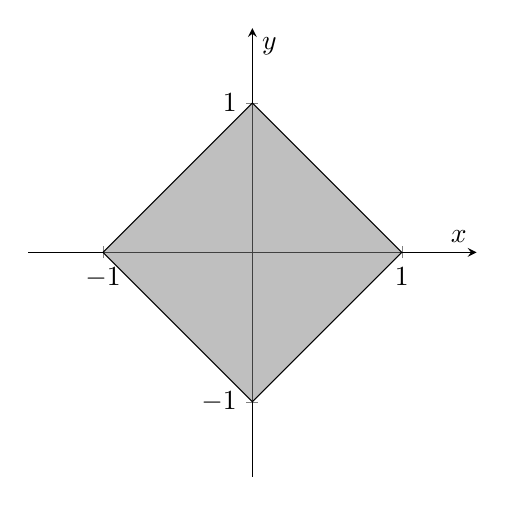
\begin{tikzpicture}
                \begin{axis}[
                    axis lines = center,
                    xlabel = $x$,
                    ylabel = $y$,
                    xmin = -1.5, xmax = 1.5,
                    ymin = -1.5, ymax = 1.5,
                    xtick = {-1,0,1},
                    ytick = {-1,0,1},
                    xticklabels = {$-1$,$0$,$1$},
                    yticklabels = {$-1$,$0$,$1$},
                    axis equal image
                ]
                    \addplot [
                        fill=gray,
                        fill opacity=0.5
                    ] coordinates {
                        (1,0) (0,1) (-1,0) (0,-1)
                    } -- cycle;
                \end{axis}
            \end{tikzpicture}
        \end{figure}

        Calculamos cada una de las funciones de densidad marginales:
        \begin{itemize}
            \item $f_X$ si $x \in [-1,0]$:
            \begin{equation*}
                f_X(x) = \int_{-x-1}^{x+1} \frac{1}{2} ~d{y} = \left[\frac{1}{2}y\right]_{-x-1}^{x+1} = \frac{1}{2}(x+1) - \frac{1}{2}(-x-1) = x+1.
            \end{equation*}

            \item $f_X$ si $x \in [0,1]$:
            \begin{equation*}
                f_X(x) = \int_{x-1}^{-x+1} \frac{1}{2} ~d{y} = \left[\frac{1}{2}y\right]_{x-1}^{-x+1} = \frac{1}{2}(-x+1) - \frac{1}{2}(x-1) = 1-x.
            \end{equation*}

            \item $f_Y$ si $y \in [-1,0]$:
            \begin{equation*}
                f_Y(y) = \int_{-y-1}^{y+1} \frac{1}{2} ~d{x} = \left[\frac{1}{2}x\right]_{-y-1}^{y+1} = \frac{1}{2}(y+1) - \frac{1}{2}(-y-1) = y+1.
            \end{equation*}

            \item $f_Y$ si $y \in [0,1]$:
            \begin{equation*}
                f_Y(y) = \int_{y-1}^{-y+1} \frac{1}{2} ~d{x} = \left[\frac{1}{2}x\right]_{y-1}^{-y+1} = \frac{1}{2}(-y+1) - \frac{1}{2}(y-1) = 1-y.
            \end{equation*}
        \end{itemize}

        Por tanto, tenemos que las funciones de densidad marginales son:
        \begin{equation*}
            f_X(x) = 1-|x|, \quad f_Y(y) = 1-|y|.
        \end{equation*}

        Por tanto, tenemos que:
        \begin{equation*}
            f_X(x) f_Y(y) = (1-|x|)(1-|y|) = 1-|x|-|y|+|x||y| \qquad \forall x\in [-1,1], y\in [-x,x].
        \end{equation*}

        Tomando como ejemplo el origen, tenemos que:
        \begin{equation*}
            \frac{1}{2} = f(0,0) \neq f_X(0)f_Y(0) = 1.
        \end{equation*}

        \item $f(x, y) = 1$, si $(x, y)$ pertenece al cuadrado de vértices $(0,0);(0,1);(1,0);(1,1)$.
        
        El recinto descrito es:
        \begin{figure}[H]
            \centering
            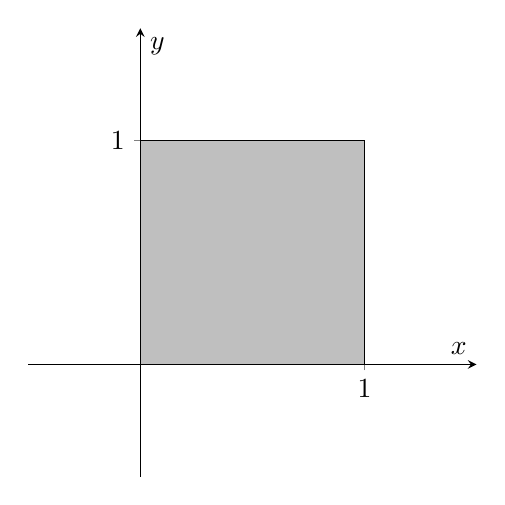
\begin{tikzpicture}
                \begin{axis}[
                    axis lines = center,
                    xlabel = $x$,
                    ylabel = $y$,
                    xmin = -0.5, xmax = 1.5,
                    ymin = -0.5, ymax = 1.5,
                    xtick = {0,1},
                    ytick = {0,1},
                    xticklabels = {$0$,$1$},
                    yticklabels = {$0$,$1$},
                    axis equal image
                ]
                    \addplot [
                        fill=gray,
                        fill opacity=0.5
                    ] coordinates {
                        (0,0) (0,1) (1,1) (1,0)
                    } -- cycle;
                \end{axis}
            \end{tikzpicture}
        \end{figure}

        Definimos funciones auxiliares:
        \Func{h_1,h_2}{\bb{R}}{\bb{R}}{t}{\begin{cases} 1 & t\in [0,1] \\ 0 & t\notin [0,1] \end{cases}}

        Tenemos que:
        \begin{equation*}
            1=f(x,y)=h_1(x)h_1(y) \qquad \forall x,y\in [0,1].
        \end{equation*}

        Por tanto, las variables $X$ e $Y$ son independientes.
    \end{enumerate}
\end{ejercicio}

\begin{ejercicio}
    Sean $X_1$ y $X_2$ variables aleatorias independientes con distribución Binomial con parámetros $n_i$, $i = 1,2$, y $p = \nicefrac{1}{2}$. Calcular la distribución de $X_1 - X_2 + n_2$.\\

    Sea $Z=X_1-X_2+n_2$. Calculamos generatriz de momentos de $Z$:
    \begin{equation*}
        M_Z(t) = E[e^{tZ}] = E[e^{t(X_1-X_2+n_2)}] = E[e^{tX_1}e^{-tX_2}e^{tn_2}] = e^{tn_2}E[e^{tX_1}e^{-tX_2}].
    \end{equation*}

    Fijado $t\in \bb{R}$, como la transformación $u\mapsto e^{tu}$ es medible, tenemos que $e^{tX_1}$ y $e^{-tX_2}$ son independientes. Por tanto, usando el Teorema de la Multiplicación de las Esperanzas, tenemos que:
    \begin{equation*}
        M_Z(t) = e^{tn_2}E[e^{tX_1}]E[e^{-tX_2}] = e^{tn_2}M_{X_1}(t)M_{X_2}(-t)
    \end{equation*}

    Usando la generatriz de momentos de la Binomial, tenemos que:
    \begin{align*}
        M_Z(t) &= e^{tn_2}\left(1+p(e^t-1)\right)^{n_1}\left(1+p(e^{-t}-1)\right)^{n_2} =\\
        &=(1+p(e^t-1))^{n_1}[e^t(1+p(e^{-t}-1))]^{n_2}=\\
        &=(1+p(e^t-1))^{n_1}(1+p(e^{t}-1))^{n_2}
        \AstIg\\&\AstIg
        (1+p(e^t-1))^{n_1+n_2}.
    \end{align*}
    donde en $(\ast)$ hemos usado que $p=\nicefrac{1}{2}$.

    Por tanto, la variable $Z$ sigue una distribución Binomial con parámetros $n_1+n_2$ y $p=\nicefrac{1}{2}$. Es decir,
    \begin{equation*}
        X_1-X_2+n_2\sim B(n_1+n_2,p).
    \end{equation*}
\end{ejercicio}

\begin{ejercicio}
    La demanda en miles de toneladas de un producto, $X$, y su precio por kilogramo en euros, $Y$, tienen por función de densidad conjunta
    \[
        f(x, y) = kx^2(1-x)^3y^3(1-y)^2, \quad x, y \in~]0,1[.
    \]
    Calcular la constante $k$ para que $f$ sea una función de densidad de probabilidad, y determinar si $X$ e $Y$ son independientes. Obtener la función de densidad de probabilidad del precio para una demanda fija.\\

    Para que $f$ sea una función de densidad de probabilidad, debe cumplir que:
    \begin{equation*}
        \int_{-\infty}^{\infty}\int_{-\infty}^{\infty} f(x,y) ~d{x}~d{y} = 1.
    \end{equation*}

    Por tanto, calculamos la constante $k$:
    \begin{align*}
        1 &= \int_{0}^{1}\int_{0}^{1} kx^2(1-x)^3y^3(1-y)^2 ~d{x}~d{y} = k\int_{0}^{1}x^2(1-x)^3 ~d{x}\int_{0}^{1}y^3(1-y)^2 ~d{y} =\\
        &= k\int_{0}^{1}x^2(1-3x+3x^2-x^3) ~d{x}\int_{0}^{1}y^3(1-2y+y^2) ~d{y} =\\
        &= k\int_{0}^{1}(x^2-3x^3+3x^4-x^5) ~d{x}\int_{0}^{1}(y^3-2y^4+y^5) ~d{y} =\\
        &= k\left[\frac{1}{3}x^3-\frac{3}{4}x^4+\frac{3}{5}x^5-\frac{1}{6}x^6\right]_{0}^{1}\left[\frac{1}{4}y^4-\frac{2}{5}y^5+\frac{1}{6}y^6\right]_{0}^{1} =\\
        &= k\left(\frac{1}{3}-\frac{3}{4}+\frac{3}{5}-\frac{1}{6}\right)\left(\frac{1}{4}-\frac{2}{5}+\frac{1}{6}\right) =\\
        &= k\cdot \frac{1}{60}\cdot \frac{1}{60} = \frac{k}{3600} \Longrightarrow k=3600.
    \end{align*}

    Comprobamos ahora si $X$ e $Y$ son independientes. Para ello, definimos funciones auxiliares:
    \Func{h_1}{\bb{R}}{\bb{R}}{x}{\begin{cases} x^2(1-x)^3 & x\in~]0,1[ \\ 0 & x\notin~]0,1[ \end{cases}}
    \Func{h_2}{\bb{R}}{\bb{R}}{y}{y^3(1-y)^2}

    Por tanto, tenemos que:
    \begin{equation*}
        f(x,y) = h_1(x)h_2(y) \qquad \forall x,y\in~\bb{R}
    \end{equation*}

    Por tanto, las variables $X$ e $Y$ son independientes. Buscamos ahora la función de densidad de probabilidad del precio para una demanda fija $D$. Para ello, como $X$ e $Y$ son independientes, tenemos que:
    \begin{align*}
        f_{Y\mid X=D}(y) &= f_Y(y) = \int_{-\infty}^{\infty} f(x,y) ~d{x} = ky^3(1-y)^2\int_{0}^{1}x^2(1-x)^3 ~d{x} =\\&= 3600\cdot y^3(1-y)^2 \cdot \dfrac{1}{60} = 60\cdot y^3(1-y)^2
    \end{align*}
\end{ejercicio}